\documentclass{beamer}
\usepackage[spanish]{babel}
\usepackage[utf8]{inputenc}
\usetheme{Berlin}
\usecolortheme{whale}
\useoutertheme{shadow}
\useinnertheme{circles}
\usepackage{nicefrac}
\setbeamertemplate{navigation symbols}{}


\title[Simulación de una Epidemia Mediante Autómatas Celulares]{Simulación de una Epidemia Mediante Autómatas Celulares}
\subtitle{Curso de Herramientas Computacionales}
\author[Jiménez, Ordóñez. Universidad Nacional de Colombia]{Julián Jiménez Cárdenas$^{1}$ y Juan Ordóñez Soto$^{1}$}
\institute{$^{1}$Curso de Herramientas Computacionales, Universidad Nacional de Colombia, Bogotá. \and \texttt{juojimenezca@unal.edu.co}\and \texttt{jsordonezs@unal.edu.co}}
\date{29 de Noviembre, 2016}

\begin{document}
	\frame{\titlepage}
	
	\begin{frame}
		\frametitle{Índice}
		\tableofcontents		
	\end{frame}
	\section{Resumen}	
	\begin{frame}
	\frametitle{Resumen}
	\begin{block}{Resumen}
	A continuación, se muestran los resultados obtenidos al reproducir el algoritmo descrito en el artículo de referencia, en éste los autores buscaban simular la evolución de una epidemia mediante difusión utilizando un objeto llamado \emph{Autómatas Celulares}, con acciones bien definidas (reglas de evolución) en cierto intervalo de tiempo. Asimismo, se comprueba la validez del método al compararlo con el modelo \textbf{SIR}, comúnmente utilizado en el modelamiento de este fenómeno.
	\end{block}
	\end{frame}
		\section{Introducción}	
	\begin{frame}
	\frametitle{Introducción}
	\begin{block}{Introducción}
	El objetivo de la simulación es reproducir el comportamiento temporal de una epidemia por difusión mediante autómatas celulares. Para ello, deben estar ubicados en un mismo punto al principio de la simulación y después irse moviendo a lo largo del espacio previamente discretizado.
	\end{block}
	\end{frame}
		\section{Algoritmo y Código}	
	\begin{frame}
\frametitle{Algoritmo}
\begin{block}{Algoritmo}

\begin{enumerate}
\item La célula rotará con igual probabilidad hacia arriba, abajo, derecha o izquierda.
\item La célula se moverá en la dirección a la cual apunta. Hay que tener precaución, pues la célula no se debe salir de los límites del mapa.


\item Si la célula está inmune sigue inmune.
\item Si está infectada se cura con probabilidad $PInm$.
\item Si está sano y tiene infectados en el mismo punto o a sus alrededores, se calcula la probabilidad que éste tiene de infectarse proporcionalmente al número de infectados alrededor suyo. Mediante dicha probabilidad se determinará si se infecta la célula o no.
\end{enumerate}
\end{block}


\end{frame}
\section{Resultados}
\begin{frame}
\begin{center}
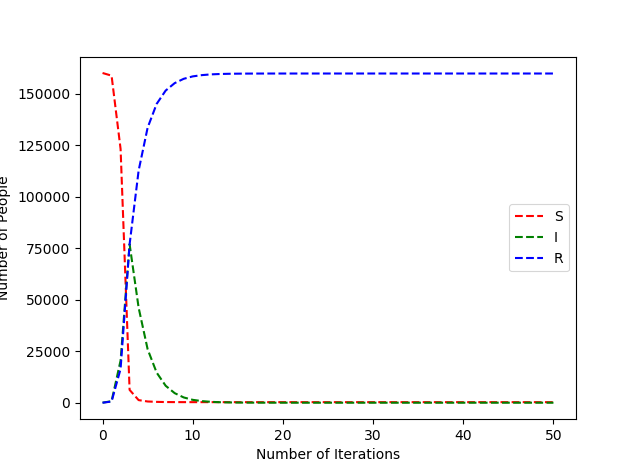
\includegraphics[width=.8\textwidth]{../article/IterationsVSNumber}
\end{center}
\end{frame}	

\begin{frame}
\begin{center}
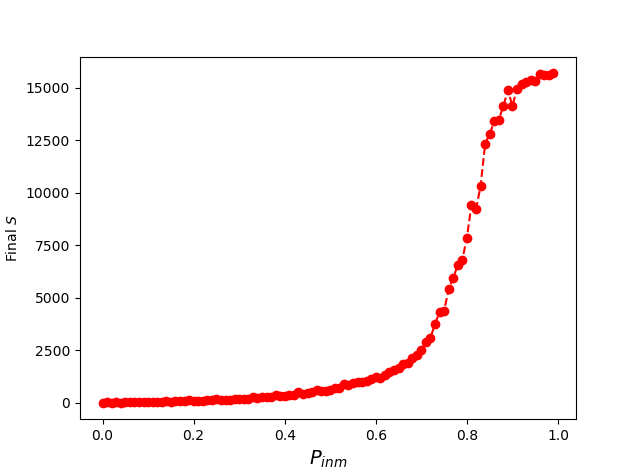
\includegraphics[width=.8\textwidth]{../article/PinmVSs}
\end{center}
\end{frame}

\begin{frame}
\begin{center}
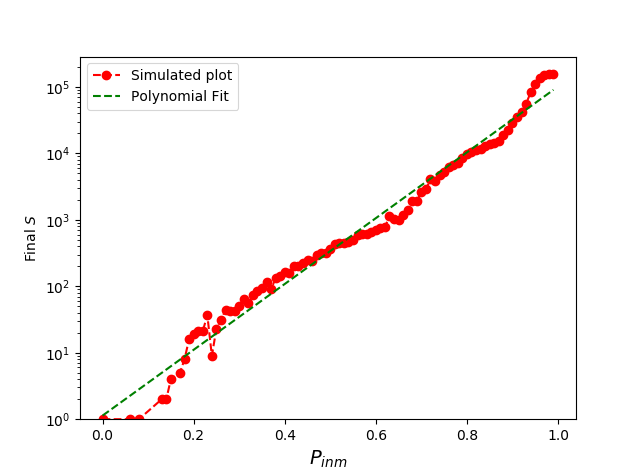
\includegraphics[width=.8\textwidth]{../article/PinmVSsSemilog}
\end{center}
\end{frame}

\section{Conclusiones}
\begin{frame}
\begin{block}{Conclusiones}
\begin{enumerate}
\item Mediante las herramientas computacionales se pueden resolver problemas que, matemáticamente suelen ser más complejos de tratar, como el modelo \textbf{SIR}. Además, es posible implementar elementos, en otro modo imposible, como por ejemplo, características demográficas.

\item Realizando la gráfica semi-logarítmica, se obtiene una ley exponencial que relaciona la probabilidad de inmunización $pInm$ con la cantidad de susceptibles final, con coeficiente $a=11.4030158925$. 
\end{enumerate}
\end{block}
\end{frame}
\end{document}
